\scanpage{161}\mspage{35}
En effet, par le cor. 2 de prop. 4.2, l'hypothèse sur $TC$ implique que $TC=\widetilde{TC}$, donc comme $TC\subset\unsure{C|TC}\cap W$, l'hypothèse $C\cap W\subset\widetilde{TC}$ $(=TC)$ équivaut à $C\cap W=TC$.

\uline{Cor. 2} : Supposons $C$ et $W$ stables par facteurs directs. Alors les conditions équivalentes de la prop. 4.3. \unsure{impliquent|équivalent} :
\figure{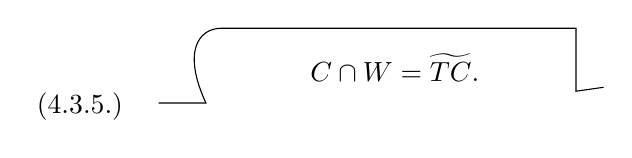
\begin{tikzpicture}
\node at (0,0) {$C\cap W=\widetilde{TC}.$};
\node at (-4,-0.5) {$(4.3.5.)$};
\draw (-3,-0.45)--(-2.4,-0.45).. controls (-2.7,0.2) and (-2.5,0.5)..(-2.2,0.5)--(2.3,0.5)--(2.3,-0.3)--(2.65,-0.25);
\end{tikzpicture}}
Dualement, si $\unsure{F|E},W$ sont stables par facteurs directs, les conditions équiv. de prop. 4.3. équivalent :
\[
F\cap W=\overline{TF}.
\tag*{(4.3.5')}
\]
En effet, si $C$ et $W$ sont stables par fact. directs, il en est de \unsure{$=$|même} de $C\cap W$, et \deleted{\unsure{comme}} dès lors si $C\cap W\subset\widetilde{TC}$, comme $C\cap W$ contient $TC$, \deleted{\unsure{donc}} on en déduit $\widetilde{C\cap W}=\widetilde{TC}$. Mais \deleted{\unsure{Comme} \unsure{et} $\unsure{C}$} Comme $C\cap W\unsure{\longleftrightarrow|\longleftarrow}TC$ et $C\cap W$ stable par facteurs directs, $C\cap W$ est clos : \unsure{i.e.} \deleted{\unsure{donc}} $C\cap W=\widetilde{C\cap W}$, par cor. 2 de prop. \unsure{4.2|4.3}, d'où $C\cap W=\widetilde{TC}$, qed.

\uline{Cor. 3} Supposons les conditions équivalentes \inserted{a) à c)} de prop. 4.3. satisfaites, et de plus \uline{$W$ stable par facteurs directs.}\textsuperscript{*} Alors les conditions préliminaires (4.3.1) et (4.3.2) restent satisfaites quand on remplace $(C,TF)$ et $(TC,F)$, par leurs clôtures \inserted{$(C',TF')=$} $(\unsure{\overline C|\widetilde C},\overline{TF})$ et \inserted{$(TC',F')=$} $(\widetilde{TC},\overline F)$, et les conditions \deleted{\unsure{analogues|équivalentes}} équivalentes de la prop. 4.3 sont \inserted{encore} satisfaites par ces couples, sous les formes \unsure{finales|fortes}
\[
\left\{\begin{aligned}
C'\cap W&=TC'\ (=\widetilde{TC}')\\
F'\cap W&=TF'\ (=\overline{TF}')\\
W&=TF'\circ TC'.
\end{aligned}\right.
\tag*{(4.3.6)}
\]
% margin note written slanted
\margin{* En fait, il suffit de supposer \unsure{que les|que l'on} \inserted{$W\supset\widetilde{TC},\overline{TF},$} \unsure{que tout|qui sont} facteur direct d'un élément de $W$ qui est soit dans $C$, soit dans $F$, est encore dans $W$. Alors $(\widetilde C,\widetilde{TC},\unsure{\overline F|\widetilde F},\overline{TF},W)$ définissent une structure de Q. close, et on sait \unsure{que ce|que cela} implique \unsure{qu'en|qu'un} fait, $W$ \unsure{est} lui aussi \unsure{stable} par facteurs directs (4.3.\unsure{6|5}).}
% archive sheet number: 160
